\documentclass[a4paper,12pt]{article}
\usepackage{graphicx}
\usepackage{hyperref}
\usepackage[T1]{fontenc}
\usepackage[utf8]{inputenc}
\usepackage{setspace}
\usepackage[paper=a4paper,margin=1in]{geometry}

\begin{document}
	\pagenumbering{gobble}

	\begin{titlepage}

        \noindent
        \begin{minipage}[t]{0.19\textwidth}
            \vspace{-4mm}{
\includegraphics[scale=1.15]{images/logo_unimib.pdf}}
        \end{minipage}
        \begin{minipage}[t]{0.81\textwidth}
        {
                \setstretch{1.42}
                {\textsc{Università degli Studi di Milano - Bicocca}} \\
                \textbf{Scuola di Scienze} \\
                \textbf{Dipartimento di Informatica, Sistemistica e Comunicazione} \\
                \textbf{Corso di laurea in Informatica} \\
                \par
        }
        \end{minipage}

	\vspace{40mm}

	\begin{center}
            {\LARGE{
                    \setstretch{1.2}
                    \textbf{Rilevazione di eventi di Alternative Splicing \\ a partire da read paired-end}
                    \par
            }}
        \end{center}

        \vspace{50mm}

        \noindent
        {\large \textbf{Relatore:} Prof. Della Vedova Gianluca } \\

        \noindent
        {\large \textbf{Correlatore:} Prof. Rizzi Raffaella}

        \vspace{15mm}

        \begin{flushright}
            {\large \textbf{Relazione della prova finale di:}} \\
            \large{Francesco Porto} \\
            \large{Matricola 816042}
        \end{flushright}

        \vspace{40mm}
        \begin{center}
            {\large{\bf Anno Accademico 2018-2019}}
        \end{center}

        \restoregeometry

    \end{titlepage}
    
   \newpage
    
    % Abstract 
    \begin{abstract}
    In questa tesi si discuterà l'estensione di ASGAL (un tool sviluppato dall' AlgoLab in grado di rilevare eventi di Alternative Splicing)
    per il supporto alle read in formato paired-end. 
    Inizialmente verranno introdotti introdotti i concetti necessari per comprendere questo documento, oltre ad una panoramica sullo stato dell'arte.
    Verranno poi evidenziate le principali modifiche apportate ad ASGAL, ponendo l'attenzione sulle differenze tra il formato single-end e quello paired-end.
    Infine verrà mostrato un esempio di funzionamento, insieme ad alcuni possibili sviluppi futuri.
    \end{abstract}
    \newpage

		% Tavola dei contenuti
    \tableofcontents
    \newpage
    
    \pagenumbering{arabic}

		\section{Introduzione}
    	\section{Introduzione}

\subsection{ASGAL}
ASGAL (Alternative Splicing Graph ALigner) \cite{ASGAL} è un tool sviluppato dall'Algolab per l'identificazione di eventi di Alternative Splicing espressi in un campione di RNA-seq a partire da un genoma di riferimento e dall'annotazione di un gene. ASGAL si compone di quattro step:

\begin{enumerate}
	\item \textbf{Costruzione dello splicing graph}: a partire dall'annotazione di un gene e dalla genomica di riferimento, ASGAL costruisce uno splicing graph, ovvero una struttura a grafo che rappresenta tutti i trascritti noti del gene in input. Viene inoltre prodotta una linearizzazione dello splicing graph, che sarà utilizzata in fase di allineamento.
	\item \textbf{Allineamento Splice-Aware}: utilizzando l'algoritmo in \cite{MEM} ASGAL allinea le read di RNA-Seq con la linearizzazione dello splicing graph del gene in input. L'allineamento è Splice-Aware in quanto è necessario tenere traccia della posizione di esoni ed introni per un corretto allineamento.
	\item \textbf{Computazione degli allineamenti Spliced (opzionale)}: gli allineamenti prodotti dall'Allineatore Splice-Aware vengono convertiti nel formato SAM, per permetterne l'elaborazione con strumenti standard.
	\item \textbf{Rilevazione degli eventi di Alternative Splicing}: gli allineamenti prodotti dall'Allineatore Splice-Aware sono analizzati per rilevare gli eventi di Alternative Splicing indotti dalle read del campione. Gli eventi rilevati sono visualizzati in un file csv, che include diverse informazioni su ciascun evento rilevato.
\end{enumerate}

ASGAL è stato sviluppato in C++ e Python: C++ viene utilizzato nella parte di allineamento per la sua efficienza, Python nella parte di rilevazione per la sua semplicità nell'utilizzo di strutture dati complesse. Il progetto è open source, ed è disponibile su GitHub con licenza GNU v3.0. Tutti i componenti sono utilizzabili singolarmente, ma viene fornito uno script principale che ne semplifica l'utilizzo.  

Al momento ASGAL non supporta le read paired-end, un nuovo formato di read prodotte da allineatori NGS (Next Generation Sequencing), che potrebbe portare ad un incremento di efficacia ed efficienza nella rilevazione di eventi di Alternative Splicing. Nei capitoli successivi saranno descritte le principali modifiche ad esso apportate e saranno evidenziate le differenze tra i formati single-end e quelli paired-end.

L'immagine nella pagina successiva riassume il funzionamento di ASGAL.

\begin{figure}[h!]
	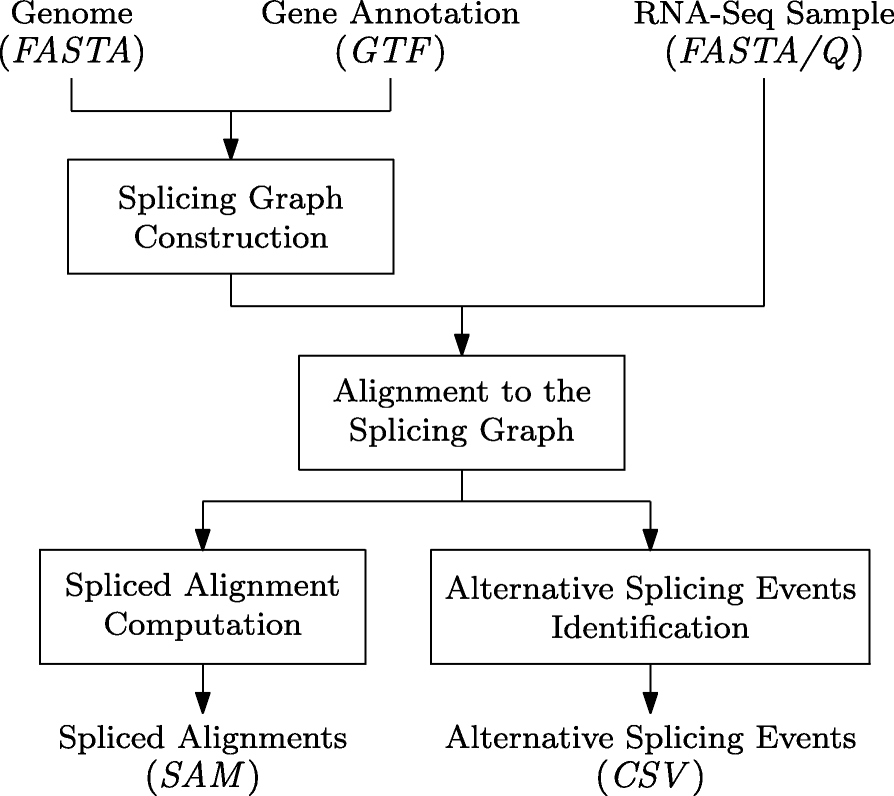
\includegraphics[width=\textwidth]{images/asgal.png}
  \caption{Il funzionamento di ASGAL illustrato}
  \label{fig:ASGAL}
\end{figure}

    	%\subsection{Paired-end Reads}
    	%\subsection{Alternative Splicing}



\end{document}
